En 2025, pour sortir le plus de performances d'un GEMM, le matériel le plus utilisé est le GPU.
Nous avons eu en cette derniere année de cours des enseignements de programmation GPU sur la plateforme CUDA (développée par NVIDIA, plus grand vendeur de cartes graphiques au monde).

Nous avons choisi d'implémenter une version CUDA du DGEMM dans le cadre de ce projet.
L'objectif initial était d'arriver à battre les performances de l'implémentation officielle de NVIDIA faisant partie de CuBLAS,
sur une architecture utilisée pour ce type de problème : Ampere datacenter (A100, Compute Capability: \textbf{SM\_80}).
Il n'y aurait pas vraiment d'intérêt à essayer de battre CuBLAS sur des cartes grand public pour lesquelles NVIDIA n'a fait aucun effort d'optimisation de la routine,
et qui par ailleurs ne possèdent pas d'unités d'accélération matériel pour les GEMM en double précision (puisqu'on serait compute bound sans efforts).

Pour ce faire, nous avons dans un premier temps implémenté un DGEMM "naïf" pour A100, puis nous avons itérativement raffiné notre noyeau jusqu'à atteindre des performances comparables à CuBLAS.

Pour toutes les implémentations CUDA du projet, nous avons utilisé la bibliothèque CuTe (faisant partie de CUTLASS\cite{?}) de NVIDIA.
Cette bibliothèque facilite les calculs d'arithmétique de pointeurs en proposant une abstraction "/texttt{Layout}" qui représente la répartition des données en mémoire de chaque matrice (A, B et C).


\subsection{Implémentation initiale ("naïve" pour \textbf{SM\_80})}
Pour implémenter un GEMM sur GPU moderne, il est très connu dans le milieu (et facilement repérable sur les specifications de la carte, voir Figure \ref{fig:a100-specs})
que les coeurs de tenseur (unités matérielles ne servant qu'à accélérer les GEMM) doivent être utilisés pour espérer atteindre les performances maximum annoncées.

\begin{figure}[H]
    \centering
    
\includegraphics[width=0.5\textwidth]{assets/dgemm_cuda/a100_specs.png}
    \caption{Spécifications de la carte A100 de NVIDIA (Figure tirée du papier "NVIDIA A100 Tensor Core GPU Architecture"\cite{?})}
    \label{fig:a100-specs}
\end{figure}

Nous avons donc choisi d'implémenter le DGEMM le plus minimal possible utilisant les tensor core double de l'architecture AMPERE (instruction /texttt{mma.sync.aligned.m8n8k4.row.col.f64.f64.f64.f64}).
Cette instruction (qui est une sortie de collective, signalé par \texttt{aligned}) requiert un bloc de 8x4 \textbf{row major} éléments de A fragmenté entre les 32 threads du WARP (groupe de 32 threads),
B pareil mais \textbf{col major} et produit en sortie un bloc de C, de taille 8x8 fragmenté entre les 32 threads du WARP,
ce schéma est détaillé Figure \ref{fig:m8n8k4}.

\begin{figure}[H]
    \centering
    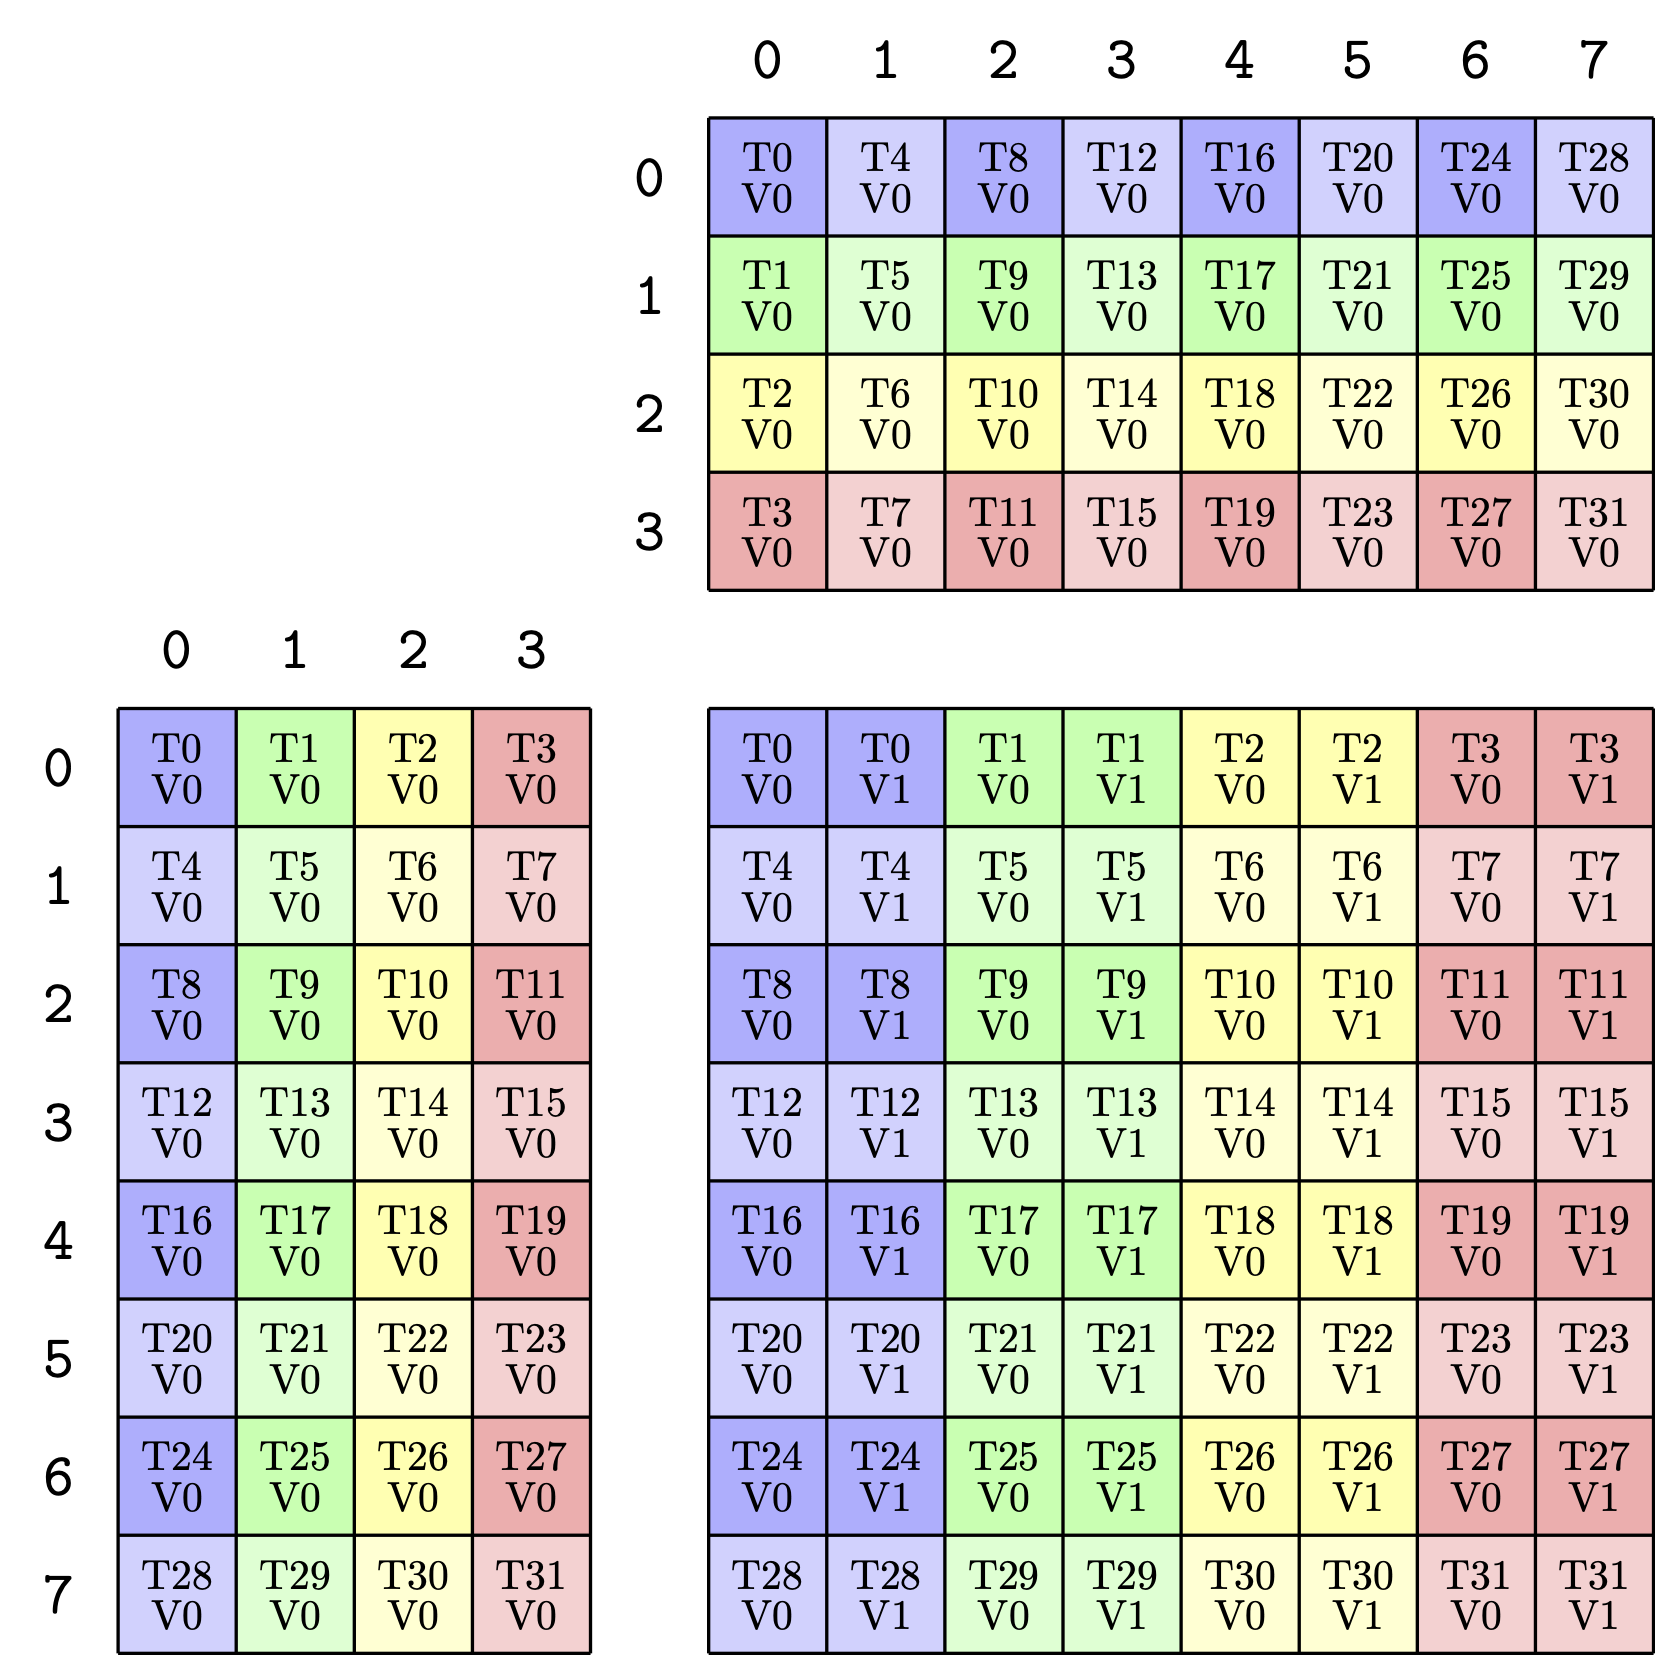
\includegraphics[width=0.5\textwidth]{assets/dgemm_cuda/m8n8k4.png}
    \caption{Schéma de l'atome CuTe \texttt{SM80\_8x8x4\_F64F64F64F64\_TN}}
    \label{fig:m8n8k4}
\end{figure}

L'algorithme utilisé dans cette implémentation est le suivant: on lance le kernel avec une taille de grille \textbf{(M/BM, N/BN)} (avec $BM$ et $BN$ les tailles de blocs sur les dimensions \texttt{M} et \texttt{N})
et une taille de bloc \textbf{(32)} (soit la taille d'un WARP, dans ce kernel, chaque bloc s'occupe de produire un bloc de taille 8x8 de la matrice de résultat C).
Chaque bloc initialise un accumulateur C (taille 8x8, fragmenté en 2 registres par thread du WARP) à zéro, copie un bloc de A et de B en mémoire partagée puis en registres (fragmenté en 1 registre double par thread)
et appelle le tensor core pour effectuer l'opération $C = A*B + C$.
Les copies de mémoire globale vers mémoire partagée pour les blocs de A et B utilisent des copies asynchrones de 64bits (1 double), cela permet juste de copie A et B en même temps mais aucun pipelining n'est réalisé.

Cette première implémentation obtient une performance très pauvre, autour de 10\% (voir Figure \ref{fig:baseline}) de CuBLAS (1,7 sur 17,3 TFlops).
\begin{figure}[H]
    \centering
    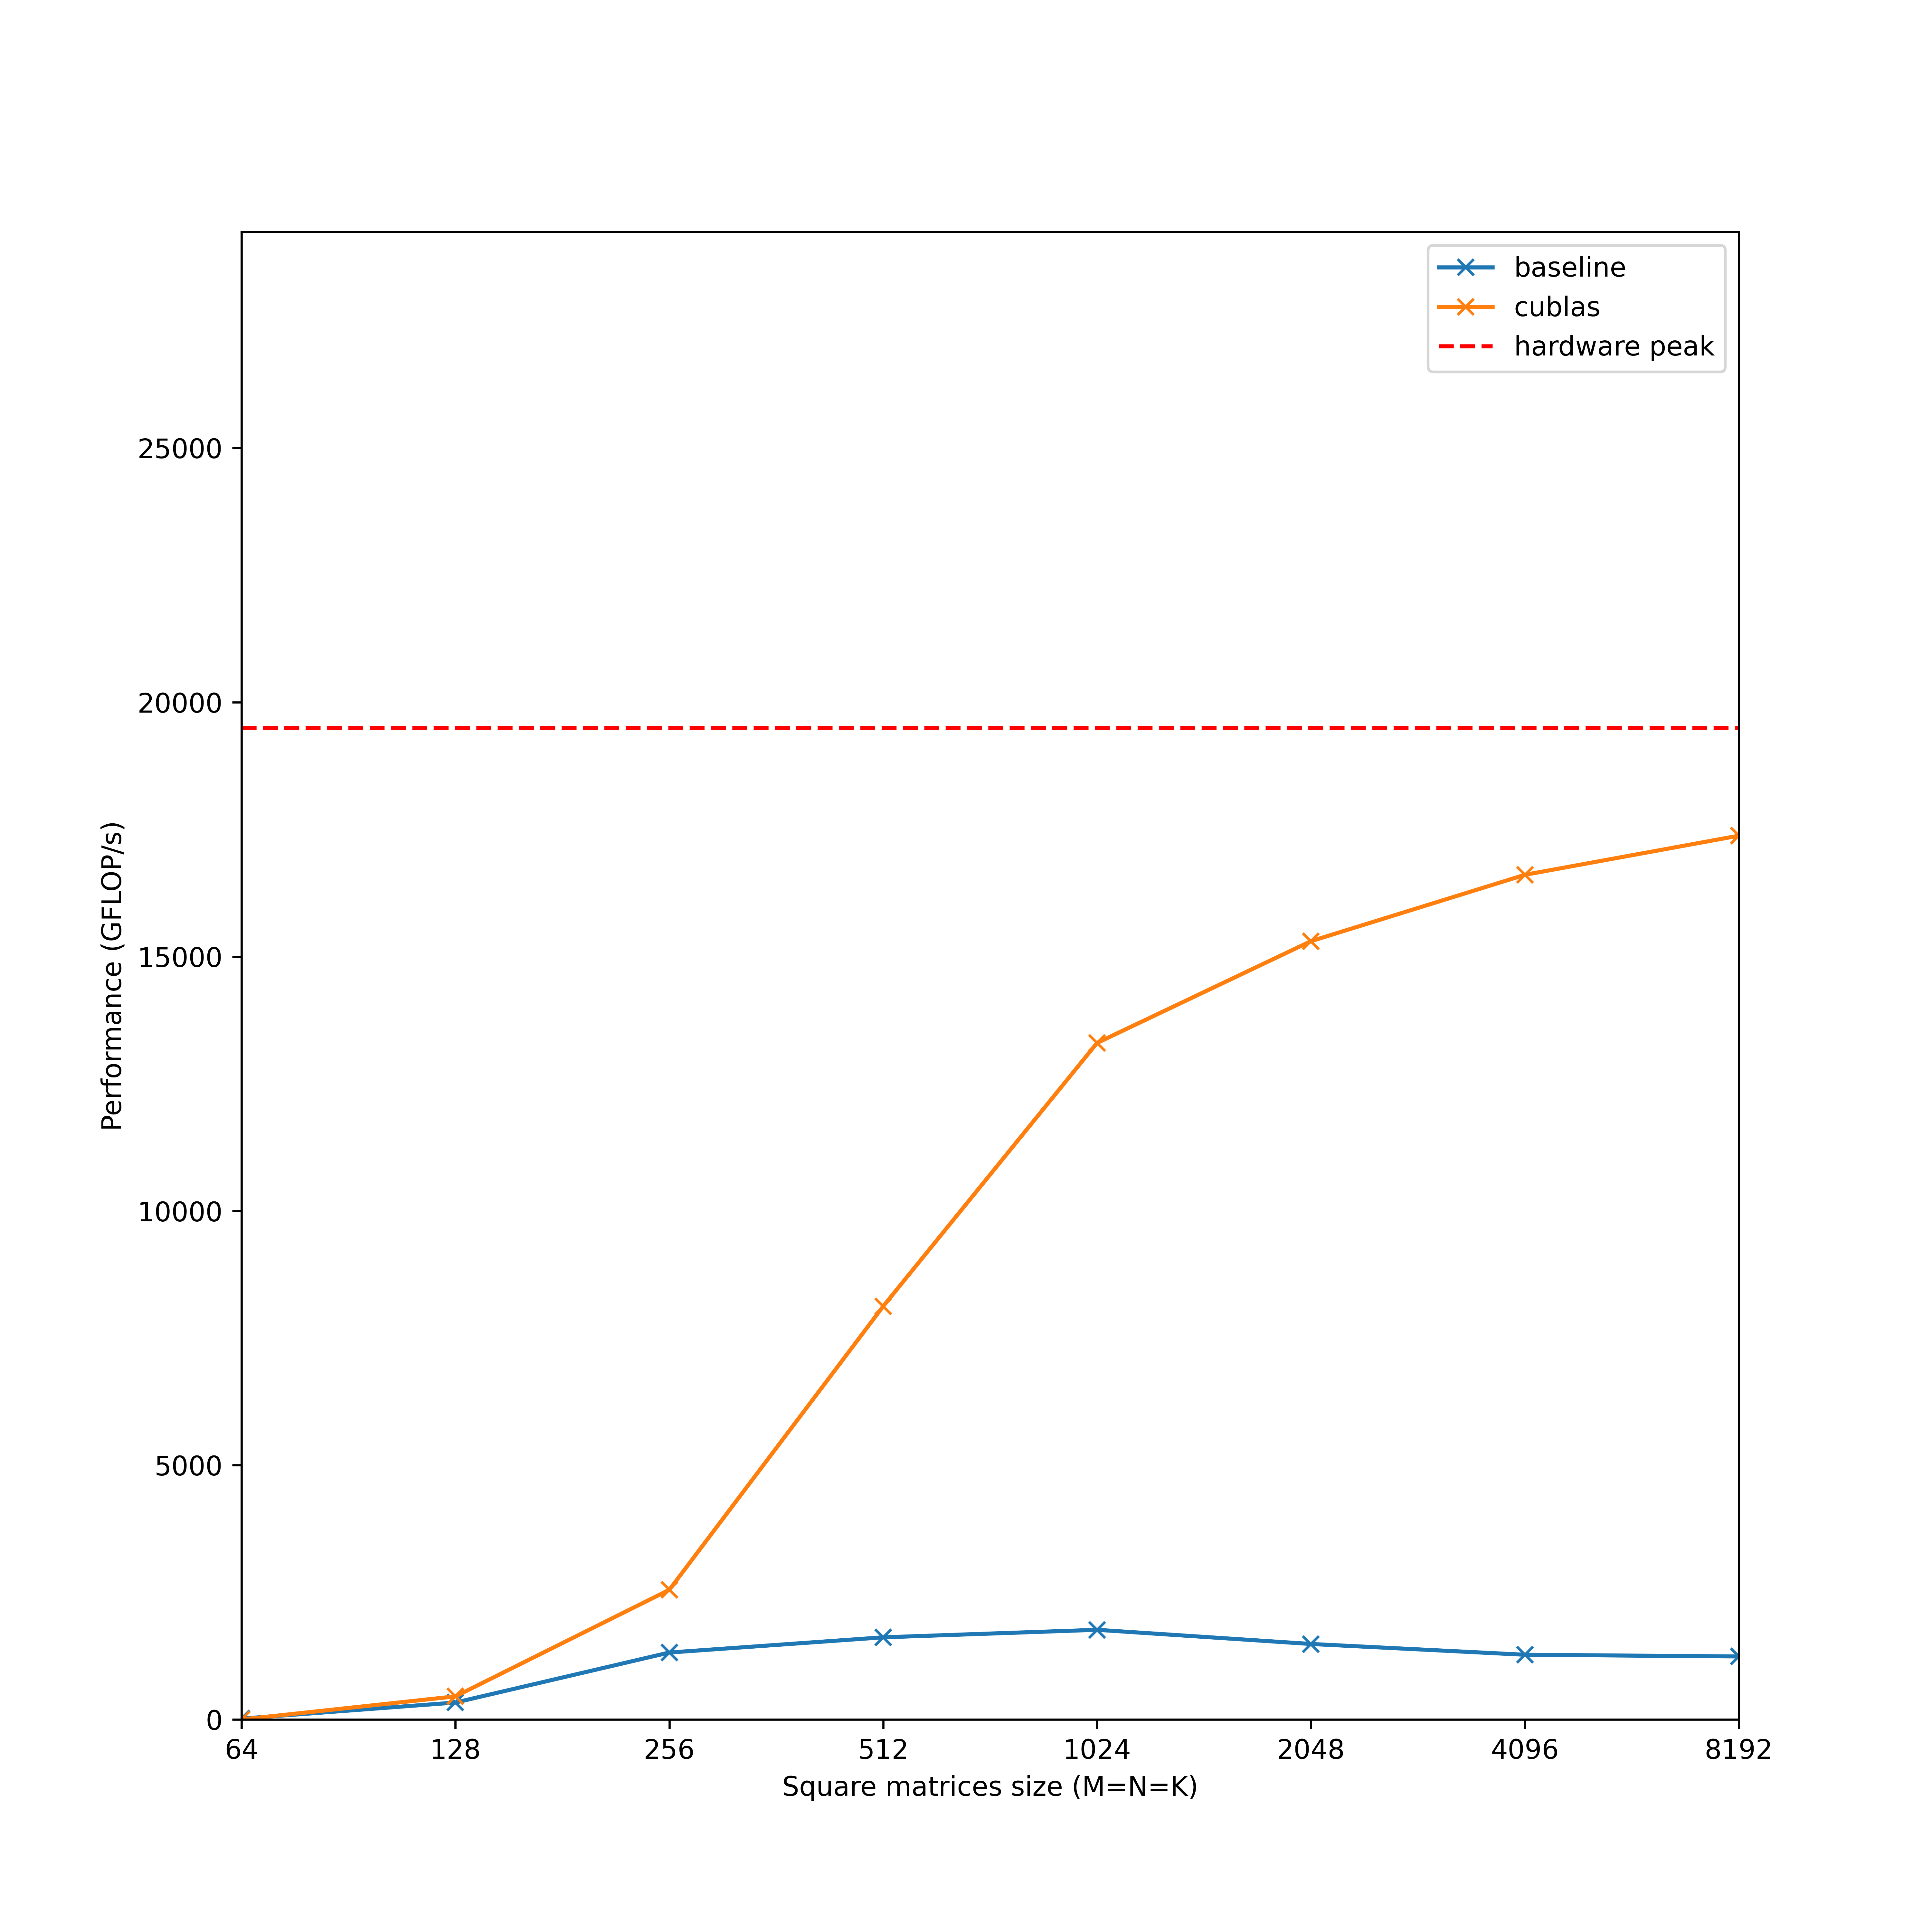
\includegraphics[width=0.5\textwidth]{assets/dgemm_cuda/cuda_baseline.png}
    \caption{Résultats de notre implémentation naïve (baseline) contre CuBLAS et la performance maximum théorique sur A100 SXM4.}
    \label{fig:baseline}
\end{figure}


\subsection{Première optimisation : agrandissement du micronoyeau}
Actuellement, notre micronoyeau fait exactement la taille de notre tensor core (8x8x4).
Pour augmenter notre intensité arithmétique, nous avons "agrandi" notre micronoyeau en apellant deux fois le tensor core sur l'axe K.

\begin{figure}[H]
    \centering
    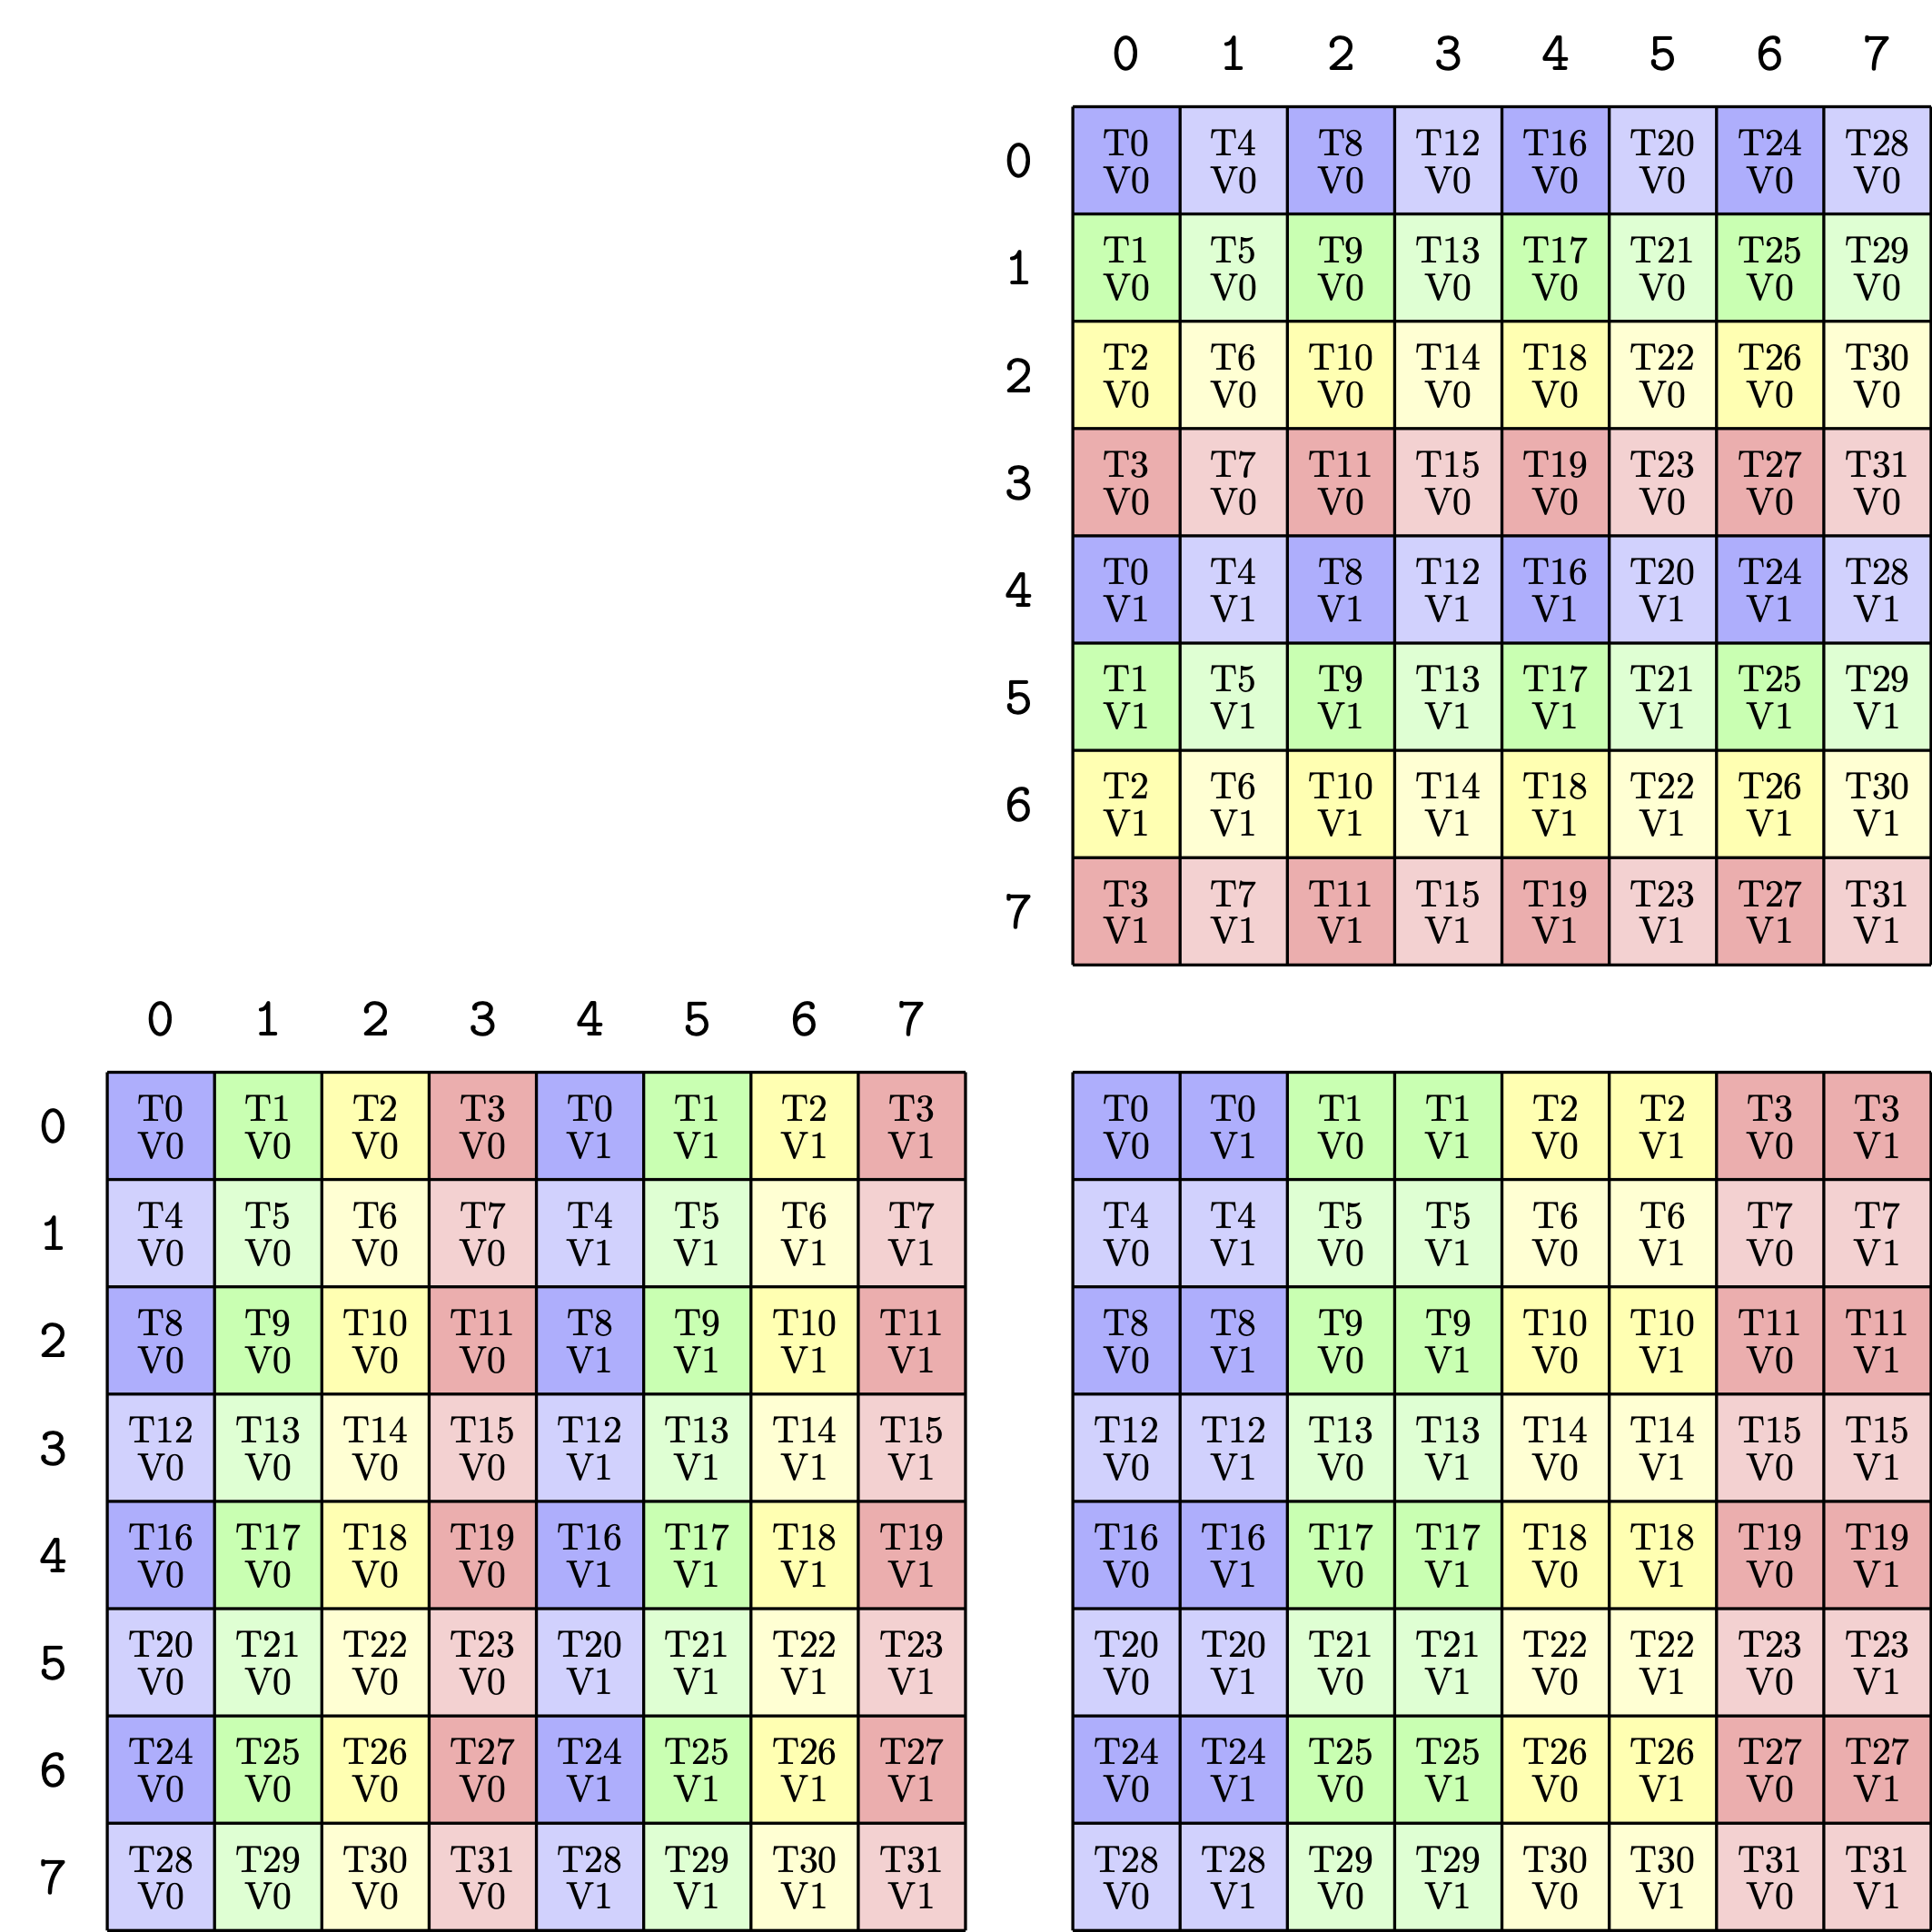
\includegraphics[width=0.5\textwidth]{assets/dgemm_cuda/m8n8k8.png}
    \caption{Schéma du TiledMMA(SM80\_8x8x4\_F64F64F64F64\_TN, Tile(8,8,8))}
    \label{fig:m8n8k8}
\end{figure}

Sur la Figure \ref{fig:m8n8k8}, on voit que nos blocs A et B sont maintenant de taille 8x8.

\begin{figure}[H]
    \centering
    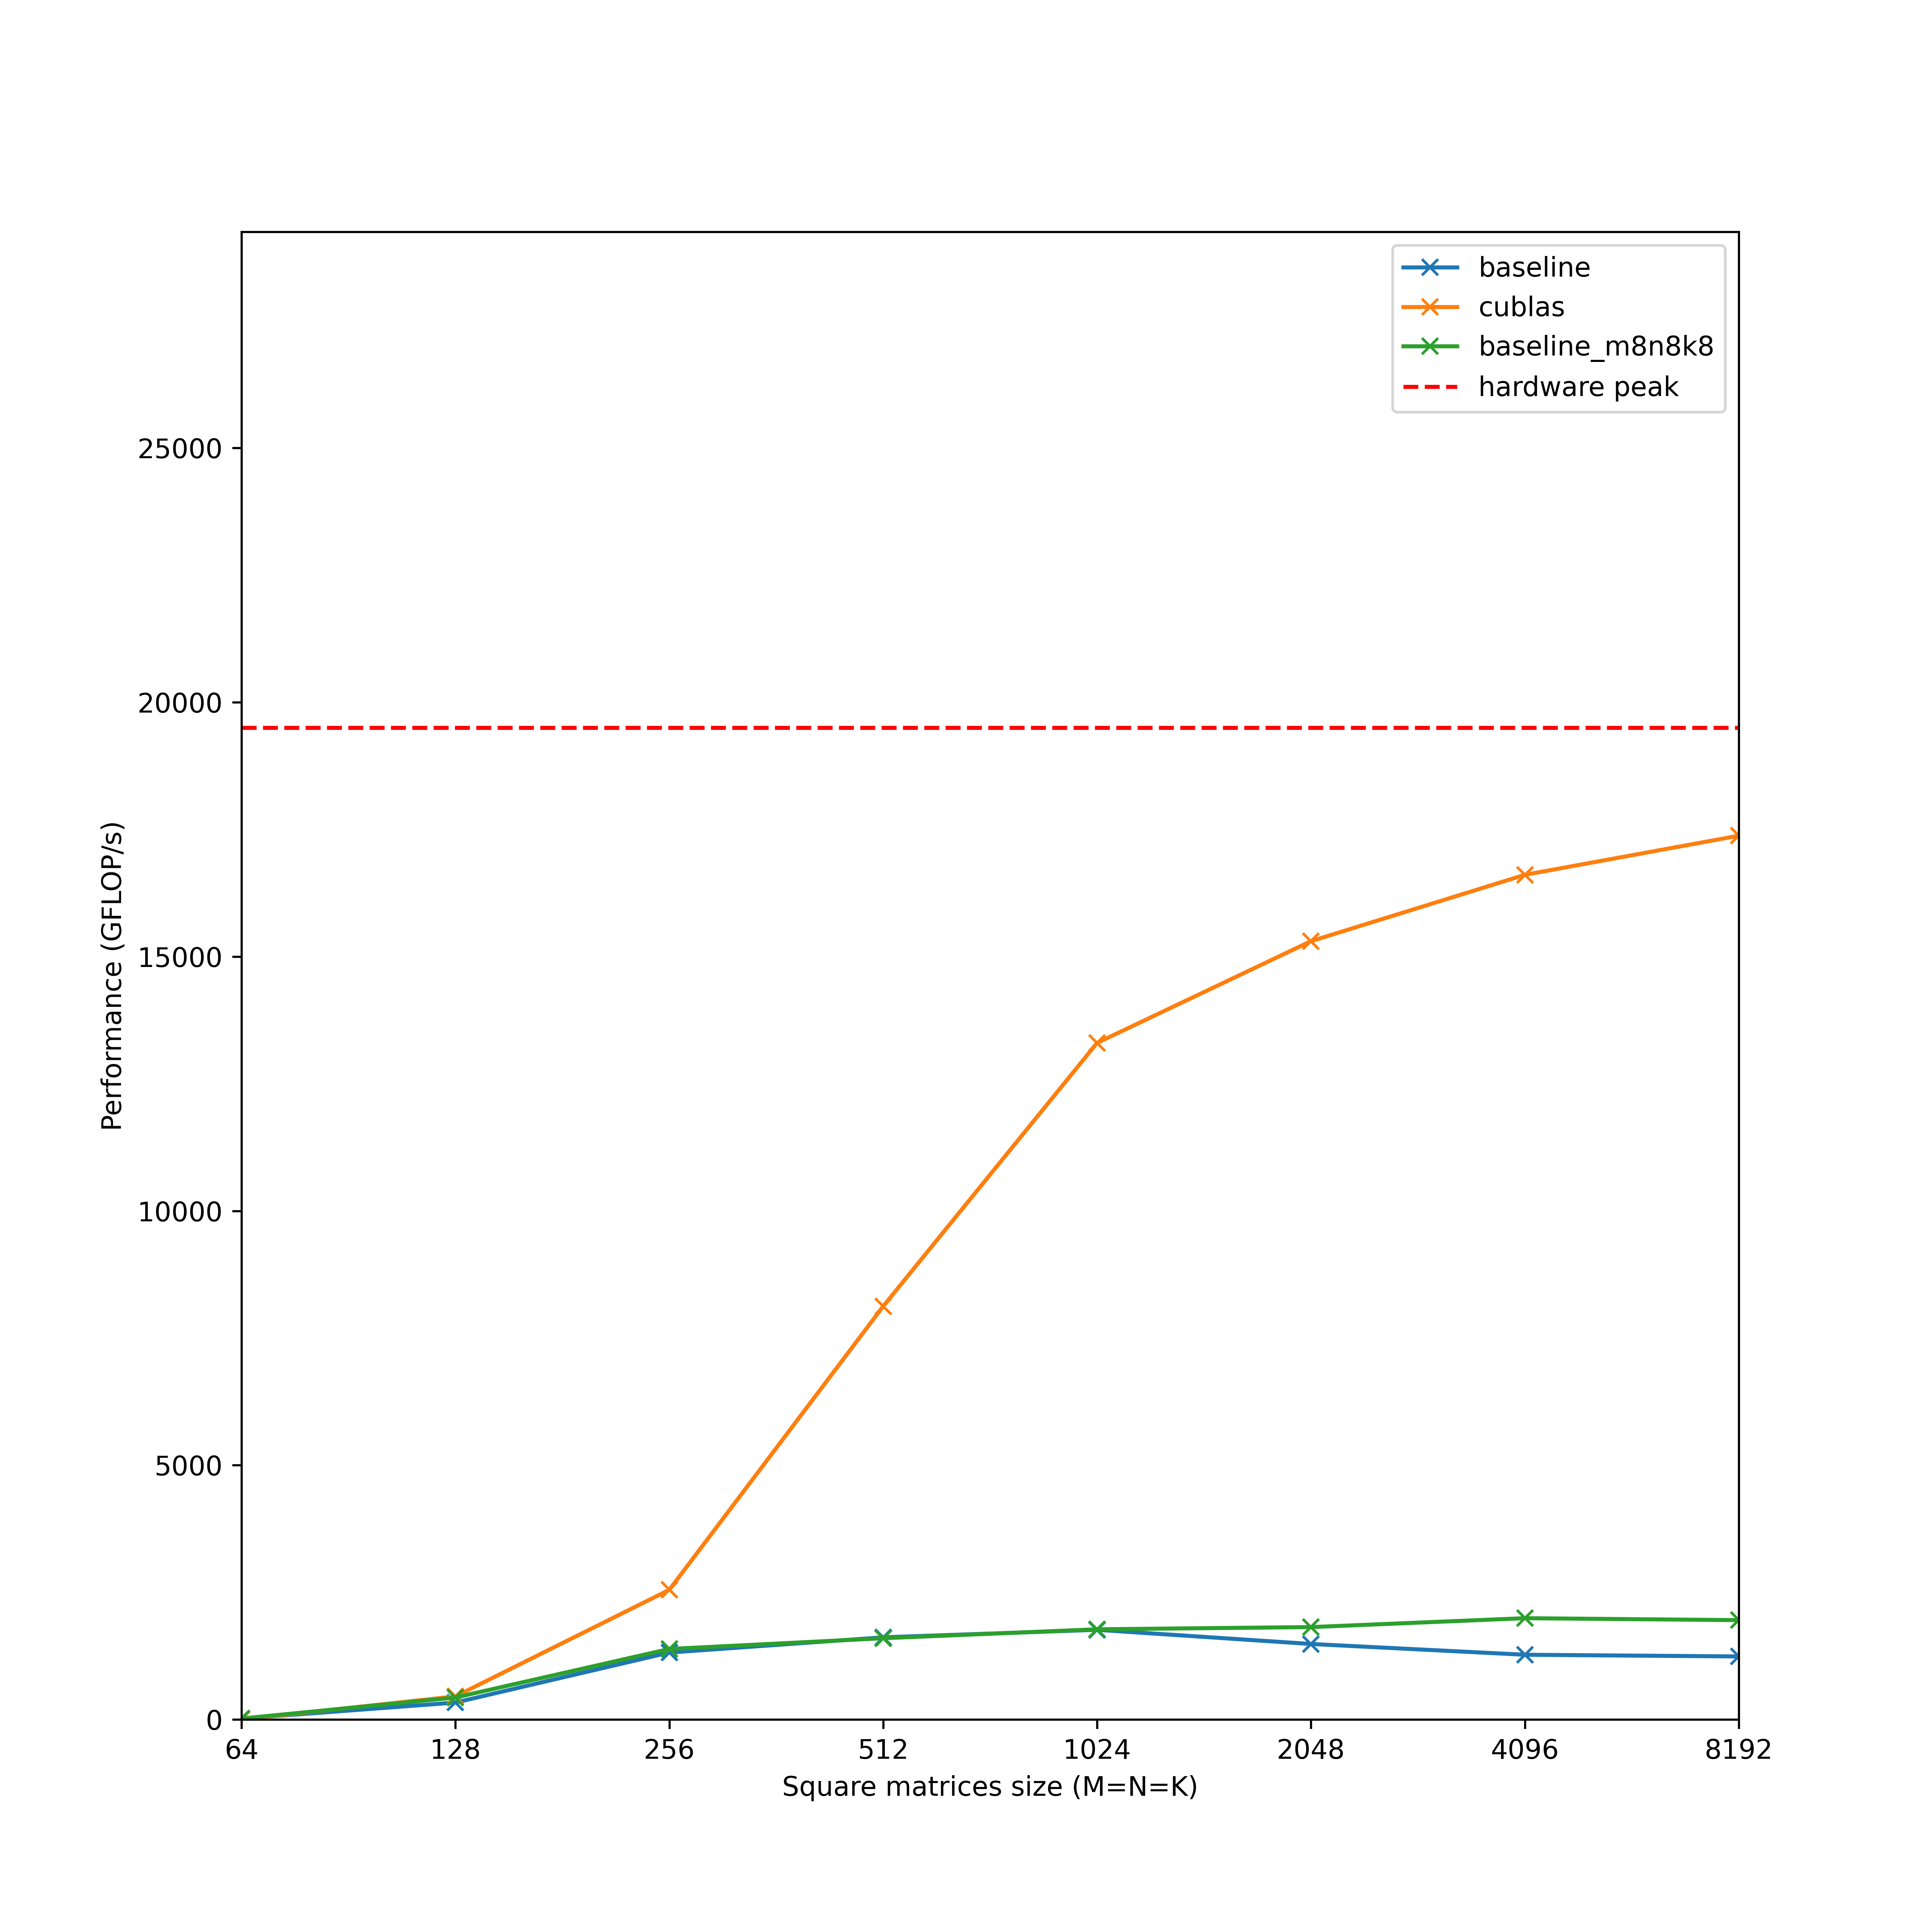
\includegraphics[width=0.5\textwidth]{assets/dgemm_cuda/cuda_baseline_m8n8k8.png}
    \caption{Résultats de l'optimisation 1 (baseline\_m8n8k8) contre CuBLAS et la performance maximum théorique sur A100 SXM4.}
    \label{fig:baseline_m8n8k8}
\end{figure}

Cette première optimisation nous amène à 11,4\% (voir Figure \ref{fig:baseline_m8n8k8}) de CuBLAS (2 sur 17,3 TFlops).


\subsection{Deuxième optimisation : copies vectorisées}
Sur notre implémentation de base "naïve", chaque thread copiait 1 double de la mémoire partagée vers un de ses registres.
Sur les GPUs NVIDIA modernes, les copies peuvent faire jusqu'à 128 bits de large (copies vectorisées).
Nous n'avions qu'un seul double à copier par thread et il nous était donc impossible d'utiliser ces copies plus larges mais maintenant,
grâce à la première optimisation, nous avons 2 doubles par bloc A/B à copier par thread de SMEM vers RMEM.

\begin{figure}[H]
    \centering
    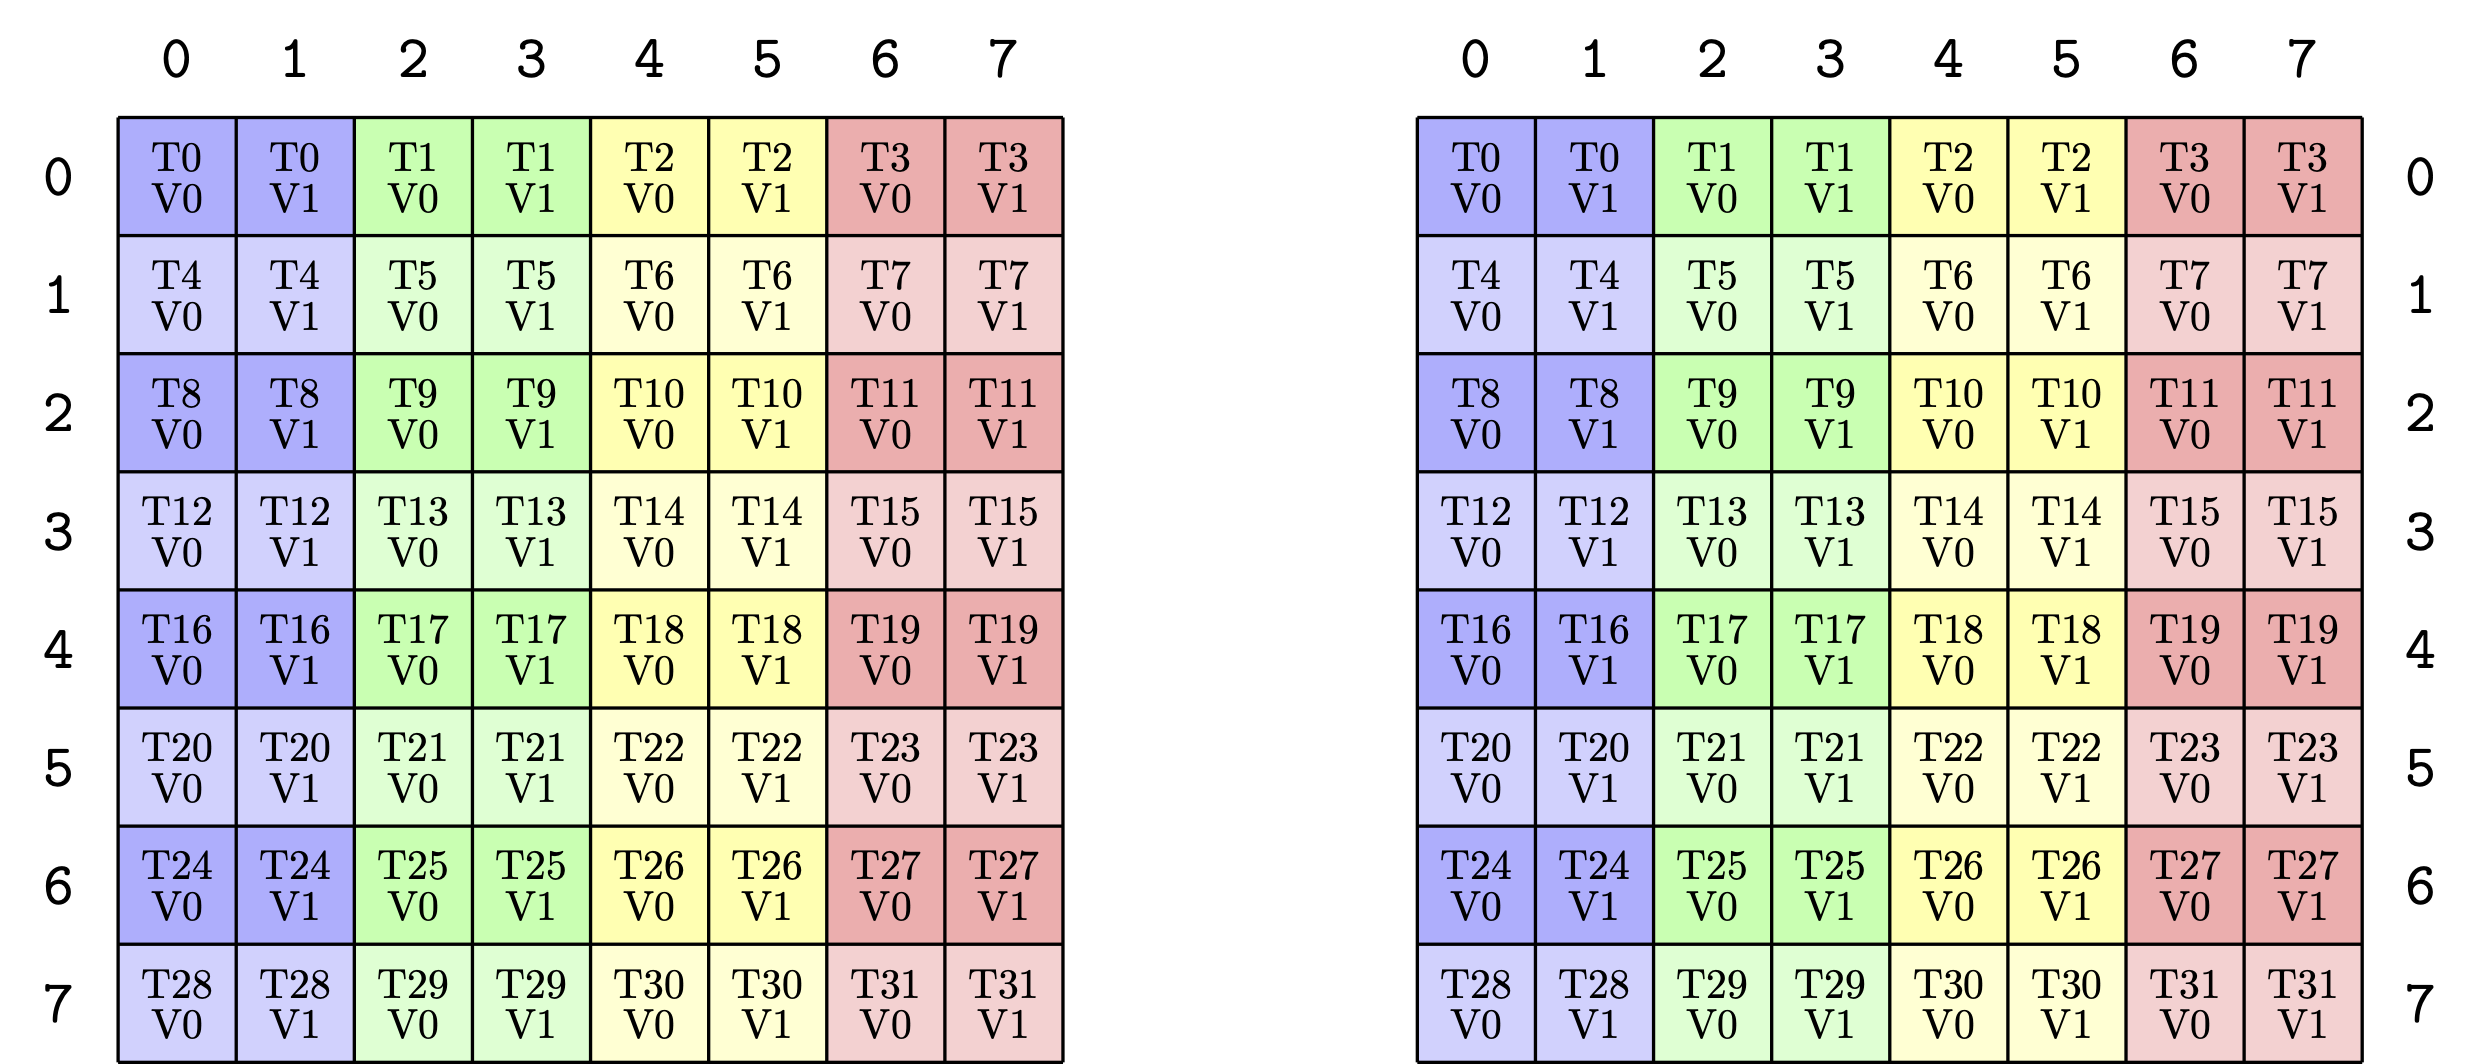
\includegraphics[width=0.5\textwidth]{assets/dgemm_cuda/128b_cpy.png}
    \caption{Schéma du partionnement d'une copie d'un block de 8x8 de la mémoire globale (GMEM) vers la mémoire partagée (SMEM) par un WARP.}
    \label{fig:128bit_copy}
\end{figure}

Sur la Figure \ref{fig:128bit_copy} on voit que les 2 élements que chaque thread copient sont contigus (pour un stockage row major).
Cela nous autorise à faire des copies de taille 128bit pour copier les deux éléments en une seule instruction.

\begin{figure}[H]
    \centering
    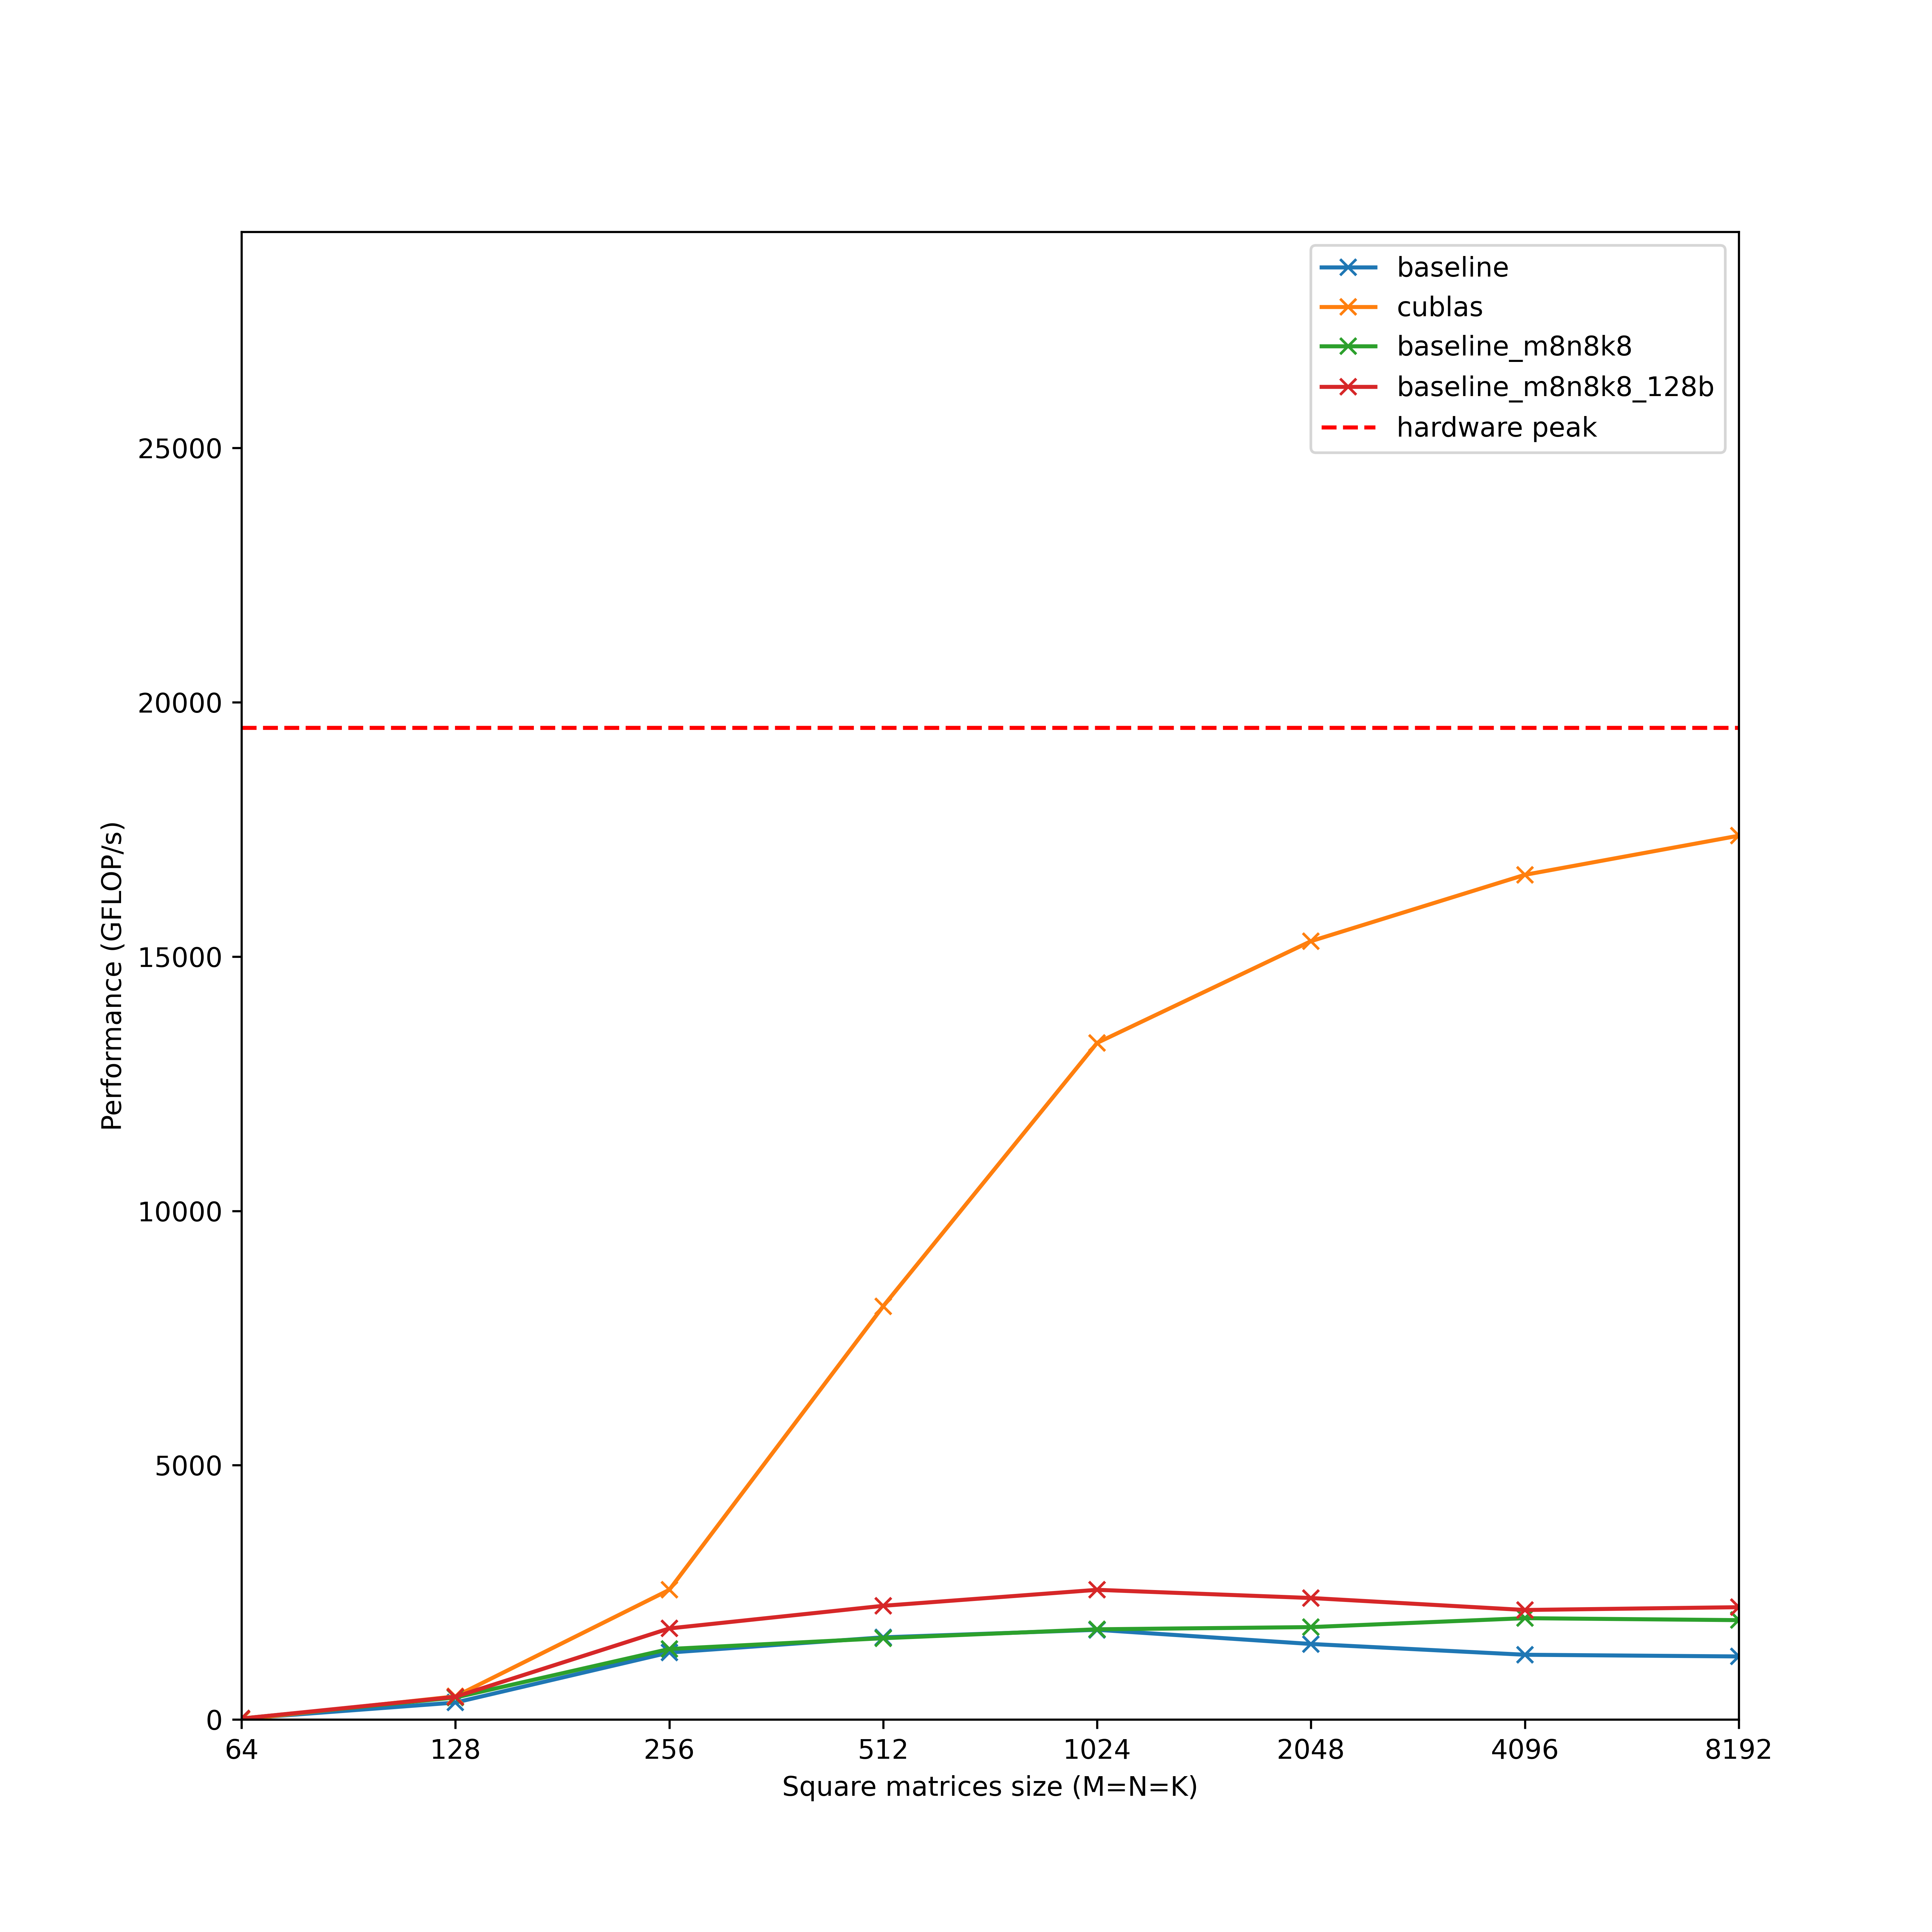
\includegraphics[width=0.5\textwidth]{assets/dgemm_cuda/cuda_baseline_m8n8k8_128b.png}
    \caption{Résultats de l'optimisation 2 (baseline\_m8n8k8\_128b) contre CuBLAS et la performance maximum théorique sur A100 SXM4.}
    \label{fig:baseline_m8n8k8_128b}
\end{figure}

Cette simple optimisation nous amène à environ 15\% (voir Figure \ref{fig:baseline_m8n8k8_128b}) de CuBLAS (2,5 sur 17,3 TFlops).


\subsection{Troisième optimisation : agrandissement du microkernel n°2}
Avec la dernière optimisation, nous utilisons assez bien le système de mémoire.
On doit maintenant essayer de faire plus de calculs avec ce qu'on arrive à charger, soit augmenter l'intensité arithmétique.

Pour se faire, on peut dupliquer notre microkernel 8 fois sur \texttt{M} et \texttt{N} et 8 fois sur \texttt{K}.
(pour trouver ces nombres nous avons fait des expériences avec une multitude de tailles différentes.)

\begin{figure}[H]
    \centering
    \includegraphics[width=0.5\textwidth]{assets/dgemm_cuda/m64n64k32.png}
    \caption{Schéma du TiledMMA(SM80\_8x8x4\_F64F64F64F64\_TN, Tile(64,64,32))}
    \label{fig:m64n64k32}
\end{figure}

On peut voir sur la Figure \ref{fig:m64n64k32} la taille des blocs A et B ainsi que du résultat C calculé par chaque WARP (et bloc pour l'instant puisqu'un bloc = 1 WARP).

\begin{figure}[H]
    \centering
    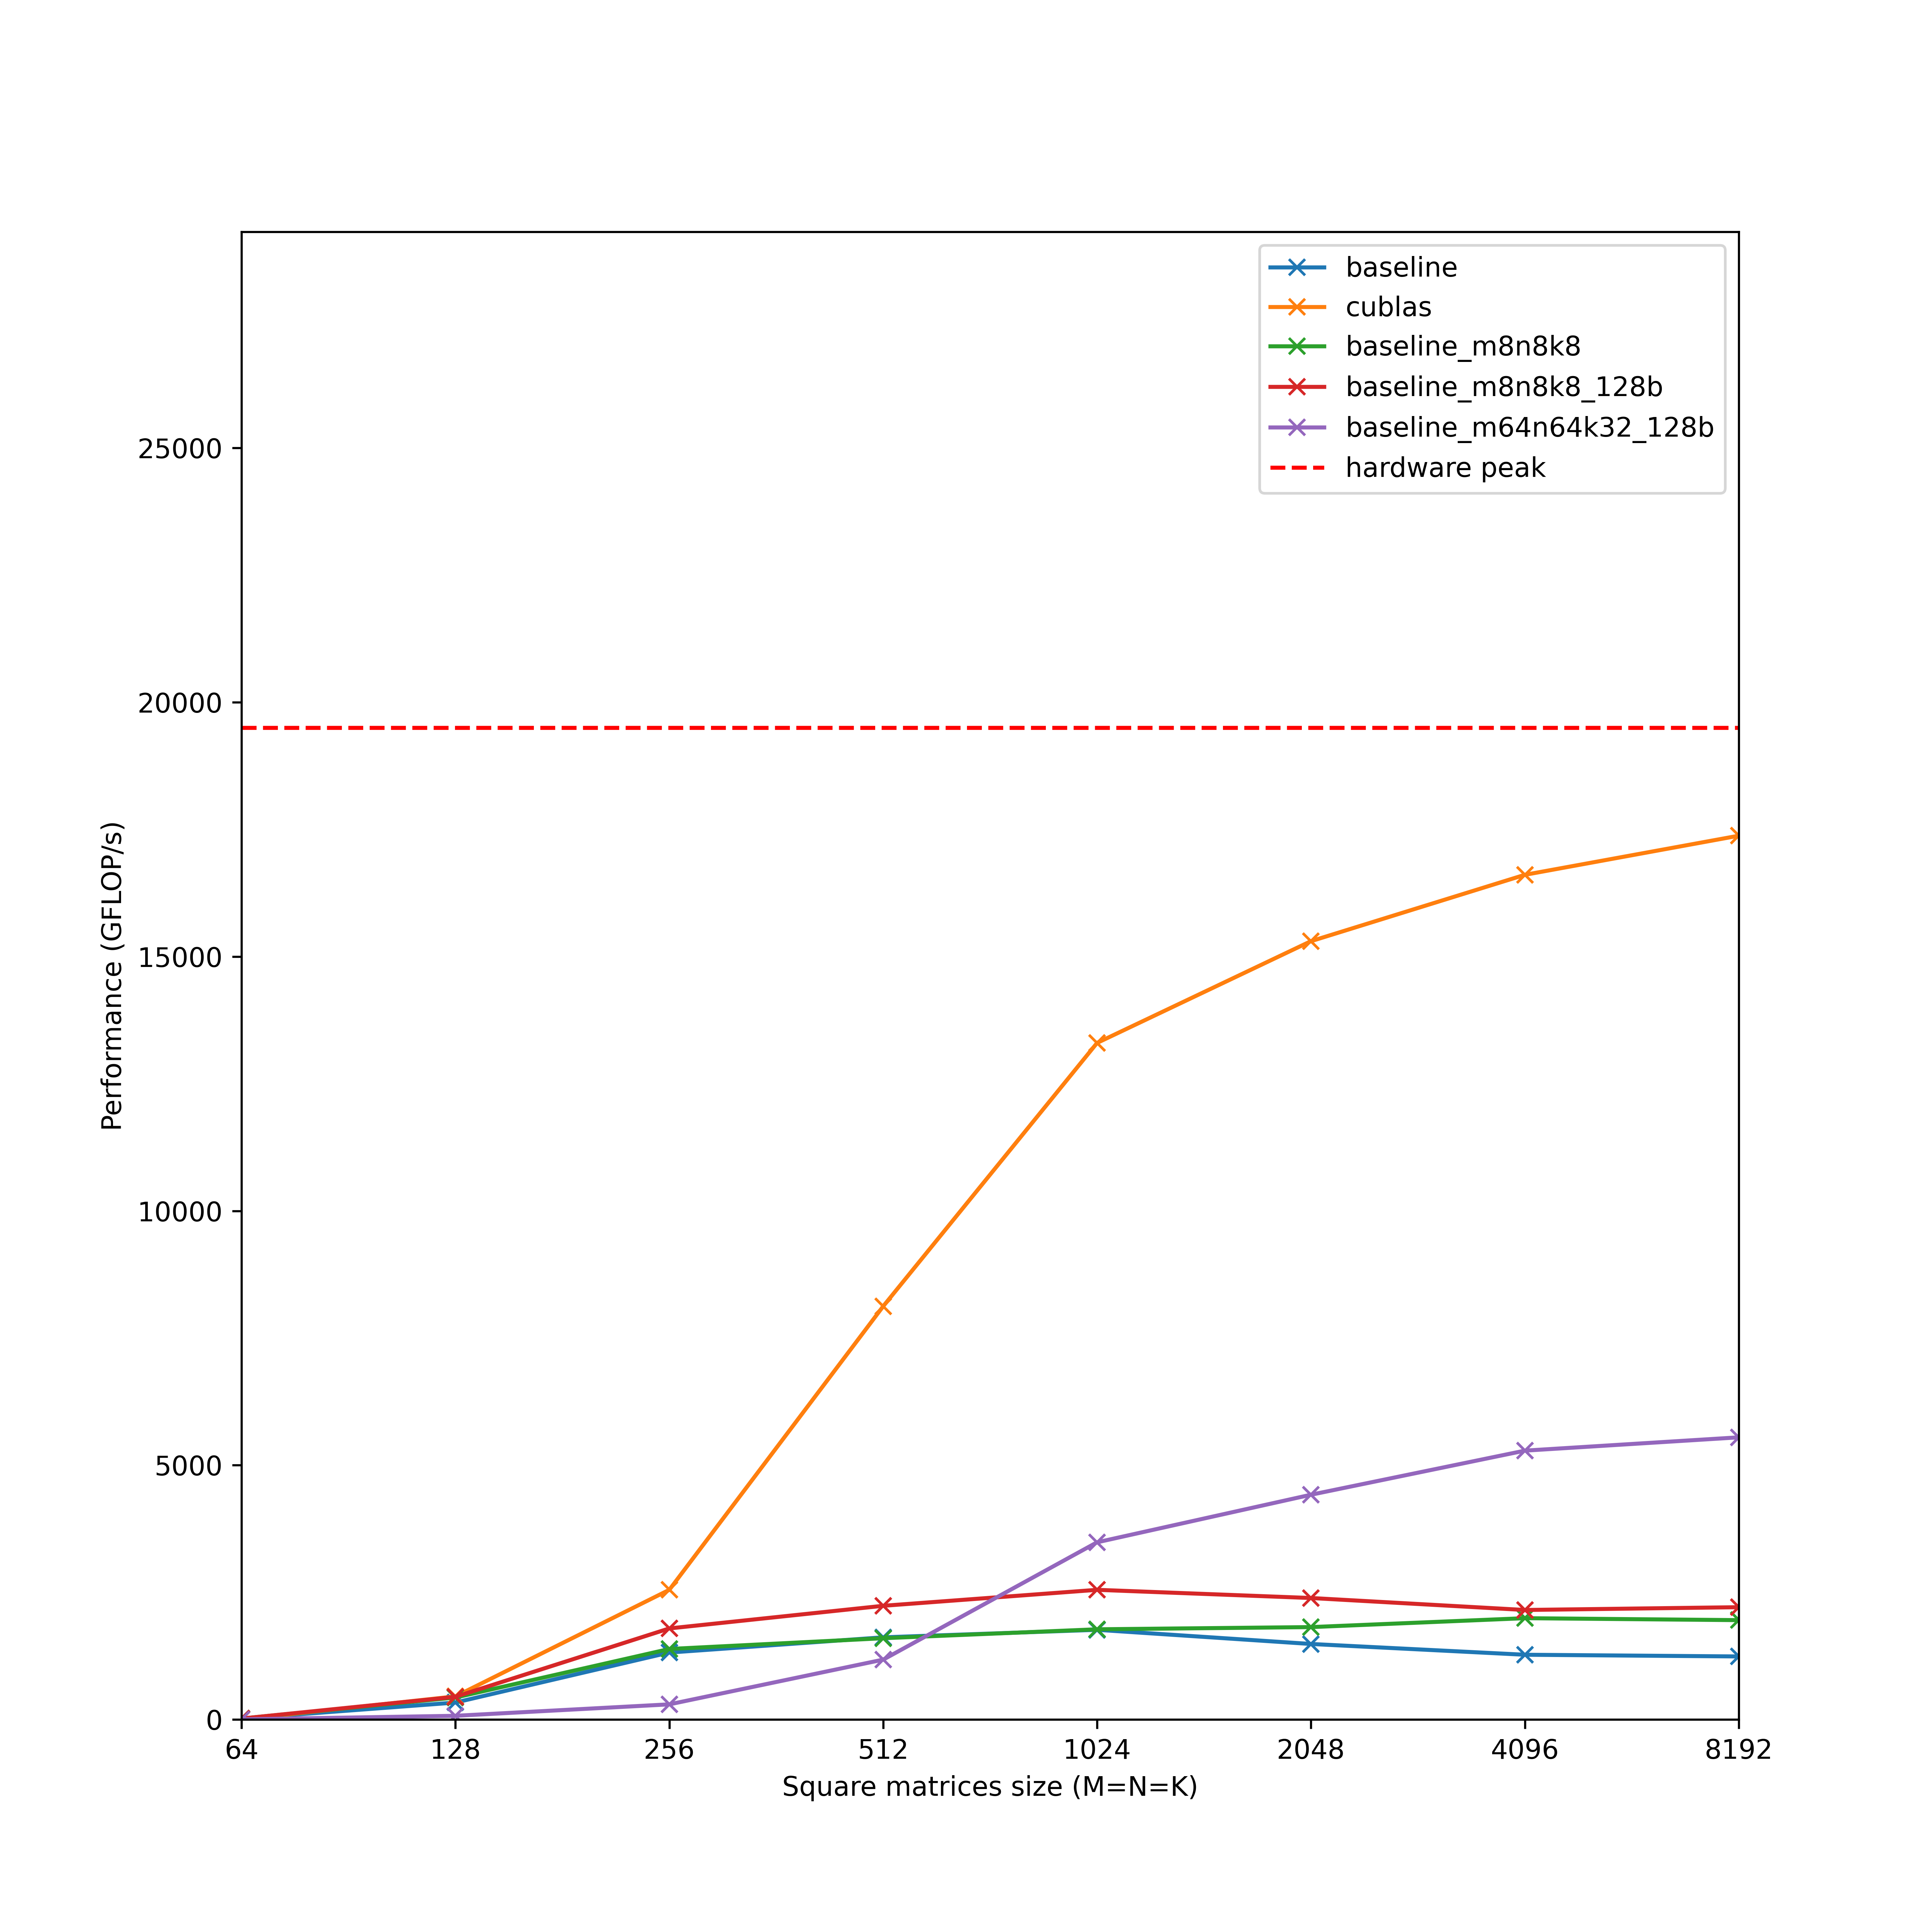
\includegraphics[width=0.5\textwidth]{assets/dgemm_cuda/cuda_baseline_m64n64k32_128b.png}
    \caption{Résultats de l'optimisation 3 (baseline\_m8n8k8\_128b) contre CuBLAS et la performance maximum théorique sur A100 SXM4.}
    \label{fig:baseline_m64n64k32_128b}
\end{figure}

Cette nouvelle taille nous permet d'atteindre 32\% (voir Figure \ref{fig:baseline_m64n64k32_128b}) de CuBLAS (5,5 sur 17,3 TFlops).


\subsection{Warptiling}

En observant le papier officiel sur la microarchitecture Ampere ("NVIDIA A100 Tensor Core GPU Architecture"\cite{?}),
on remarque qu'un SM (coeur) du GPU est composé de 4 quadrants chacun pouvant exécuter 1 instruction par cycle.

Pour maximiser notre utilisation du hardware, nous allons donc utiliser 4 WARPs par bloc et diviser notre microkernel en 4 (2 sur M et 2 sur N).

\begin{figure}[H]
    \centering
    \includegraphics[width=0.5\textwidth]{assets/dgemm_cuda/m64n64k32_4W.jpg}
    \caption{Schéma du TiledMMA(SM80\_8x8x4\_F64F64F64F64\_TN, Layout(Shape(2, 2, 1)), Tile(64,64,32))}
    \label{fig:m64n64k32_4W}
\end{figure}

\textbf{Note:} CuBLAS utilise la même taille de bloc que nous \textbf{(64,64,32)}.


Sur la Figure \ref{fig:m64n64k32_4W} on remarque que l'on utilise maintenant 128 threads pour exécuter notre microkernel.

\begin{figure}[H]
    \centering
    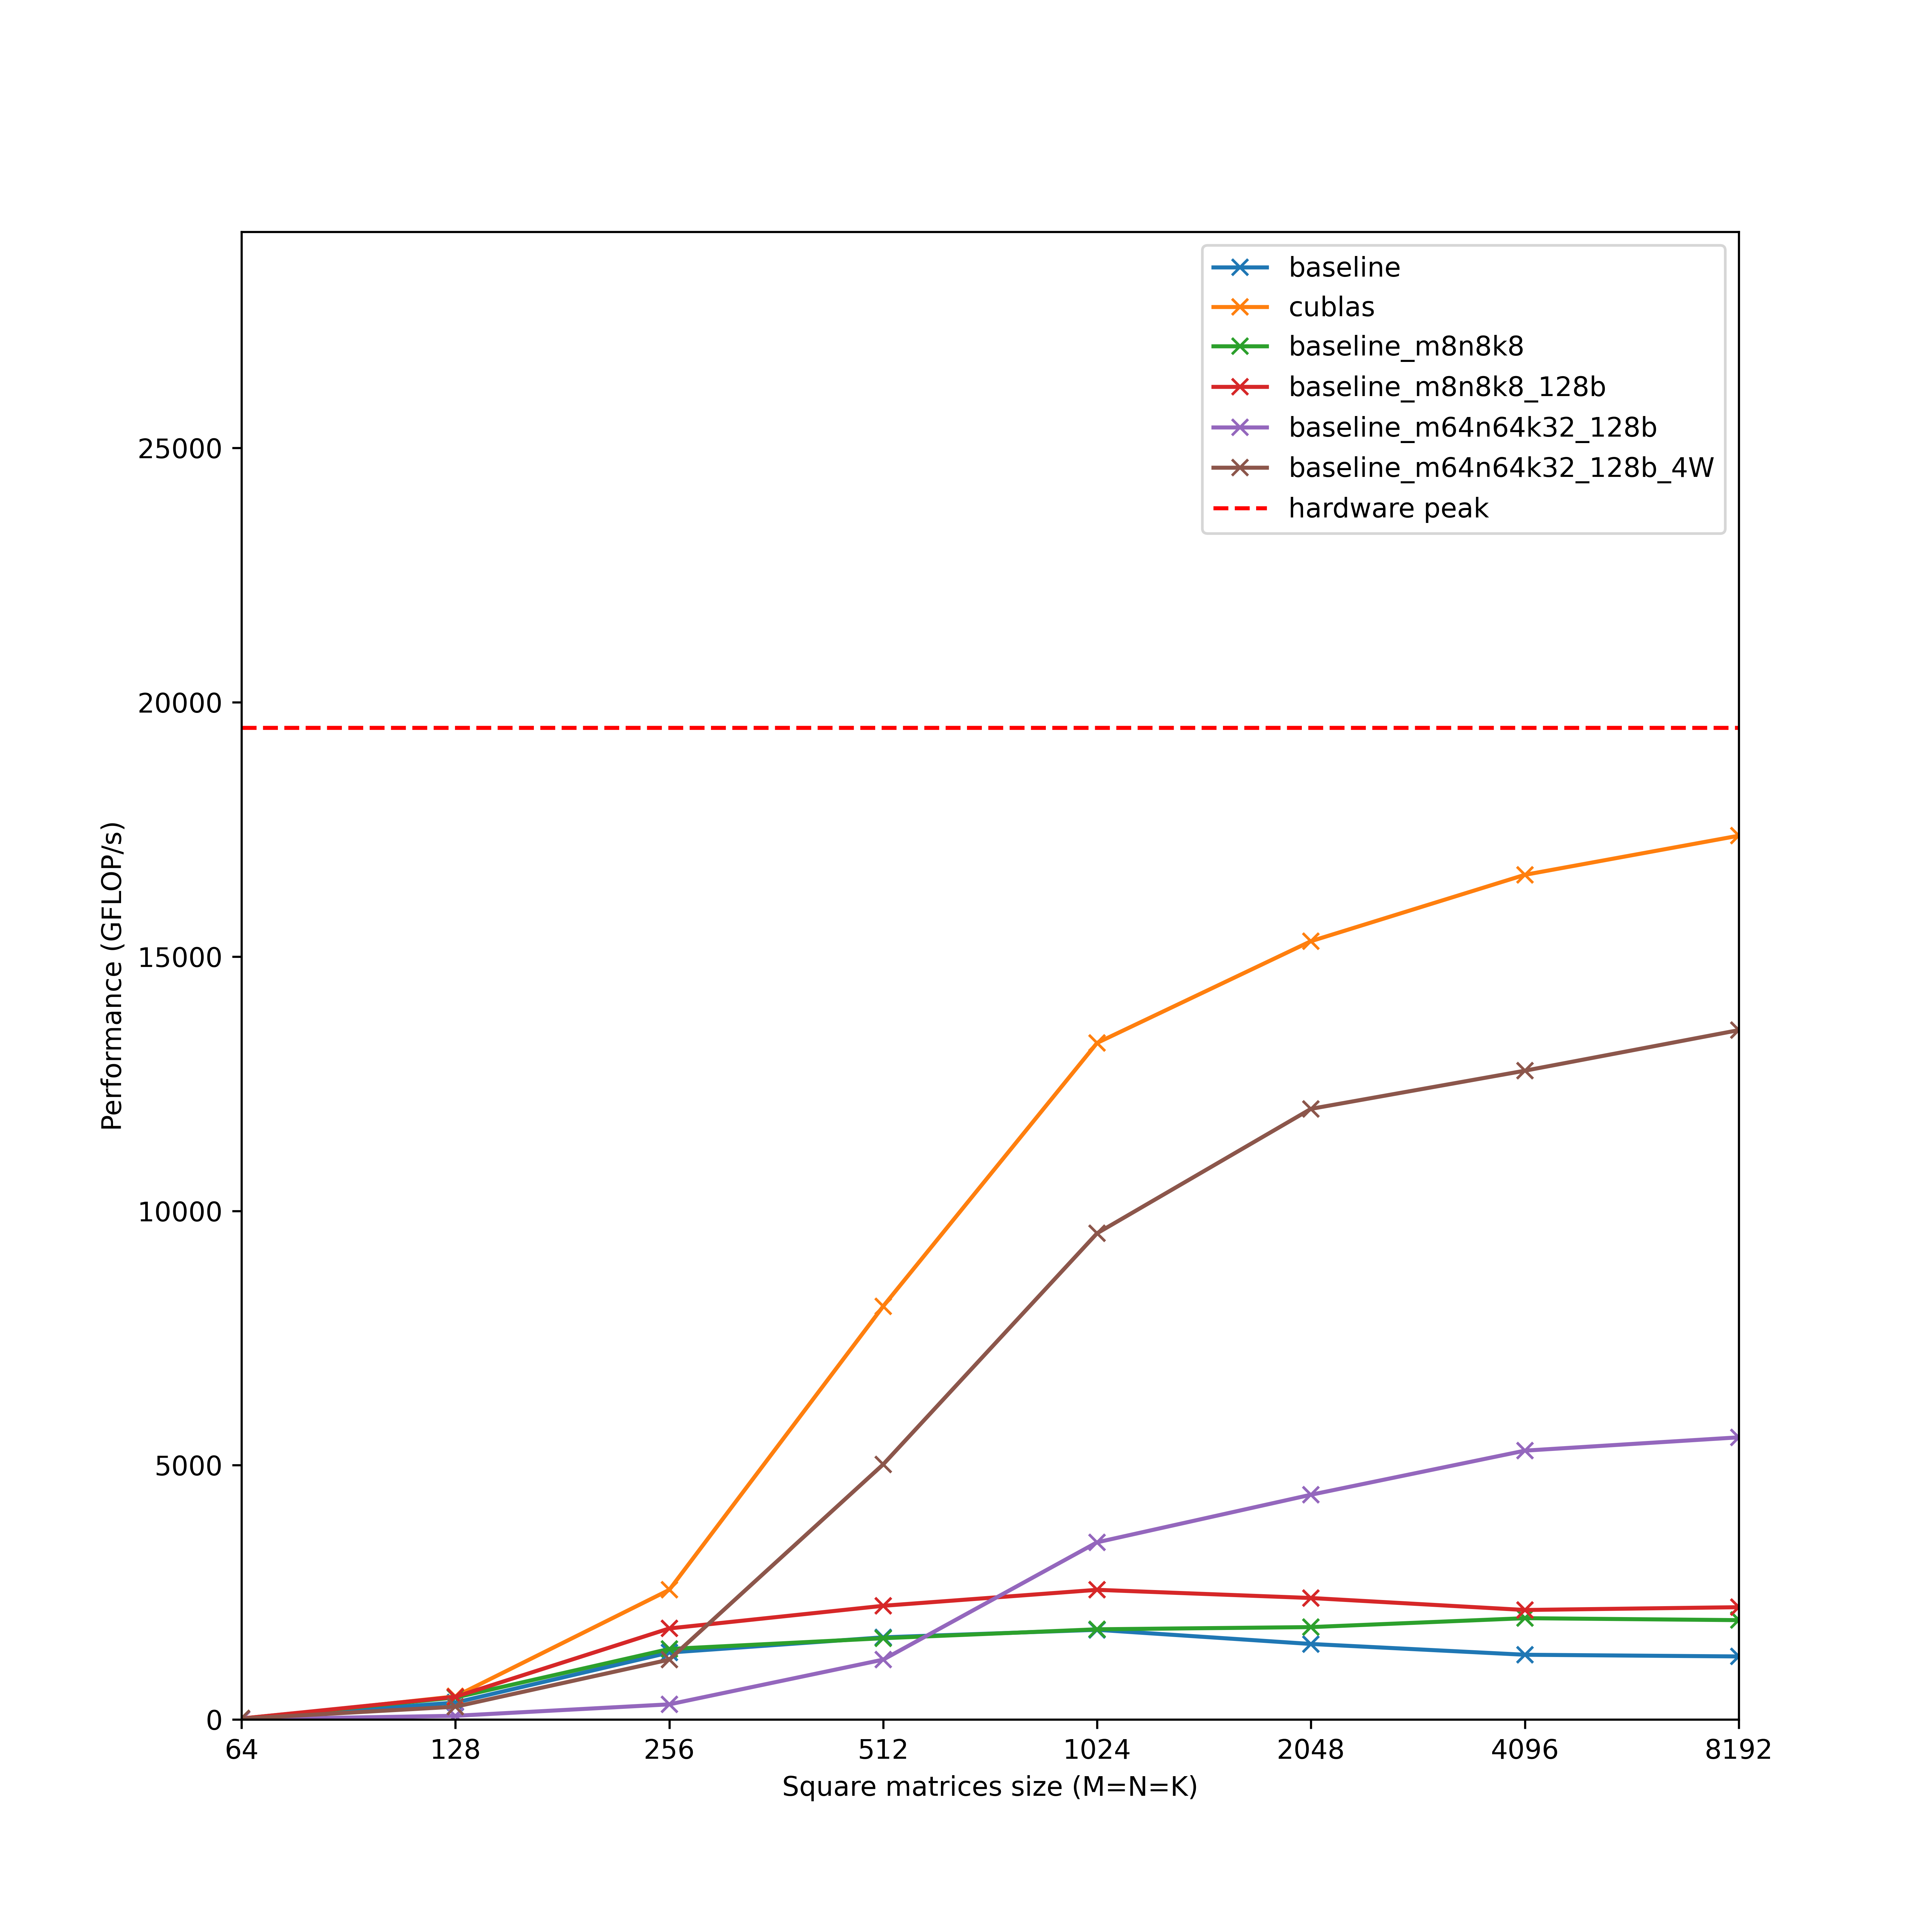
\includegraphics[width=0.5\textwidth]{assets/dgemm_cuda/cuda_baseline_m64n64k32_128b_4W.png}
    \caption{Résultats de l'optimisation 4 (baseline\_m8n8k8\_128b\_4W) contre CuBLAS et la performance maximum théorique sur A100 SXM4.}
    \label{fig:baseline_m64n64k32_128b_4W}
\end{figure}

Utiliser 4 WARPs nous amène à 78\% (voir Figure \ref{fig:baseline_m64n64k32_128b_4W}) de CuBLAS (13,6 sur 17,3 TFlops).


\subsection{Dernière optimisation : bypass le cache L1}

Depuis Ampere, des options sont ajoutables aux instructions de copie mémoire depuis la mémoire globale vers la mémoire partagée (GMEM vers SMEM) qui permettent d'instruire le hardware de ne pas "cacher" (de l'anglais to cache ..) les données copiées dans le L1.
Dans notre cas, chaque bloc chargé en SMEM n'est jamais chargé une seconde fois depuis la mémoire globale par le même SM, utiliser le L1 est alors une perte de temps.

On utilise donc la variante \texttt{cp.async.cg.shared.global} de l'instruction \texttt{cp.async} (\texttt{.cg} veut dire "cache global" soit "on ne cache que au global" donc L2 et pas L1.).

\begin{figure}[H]
    \centering
    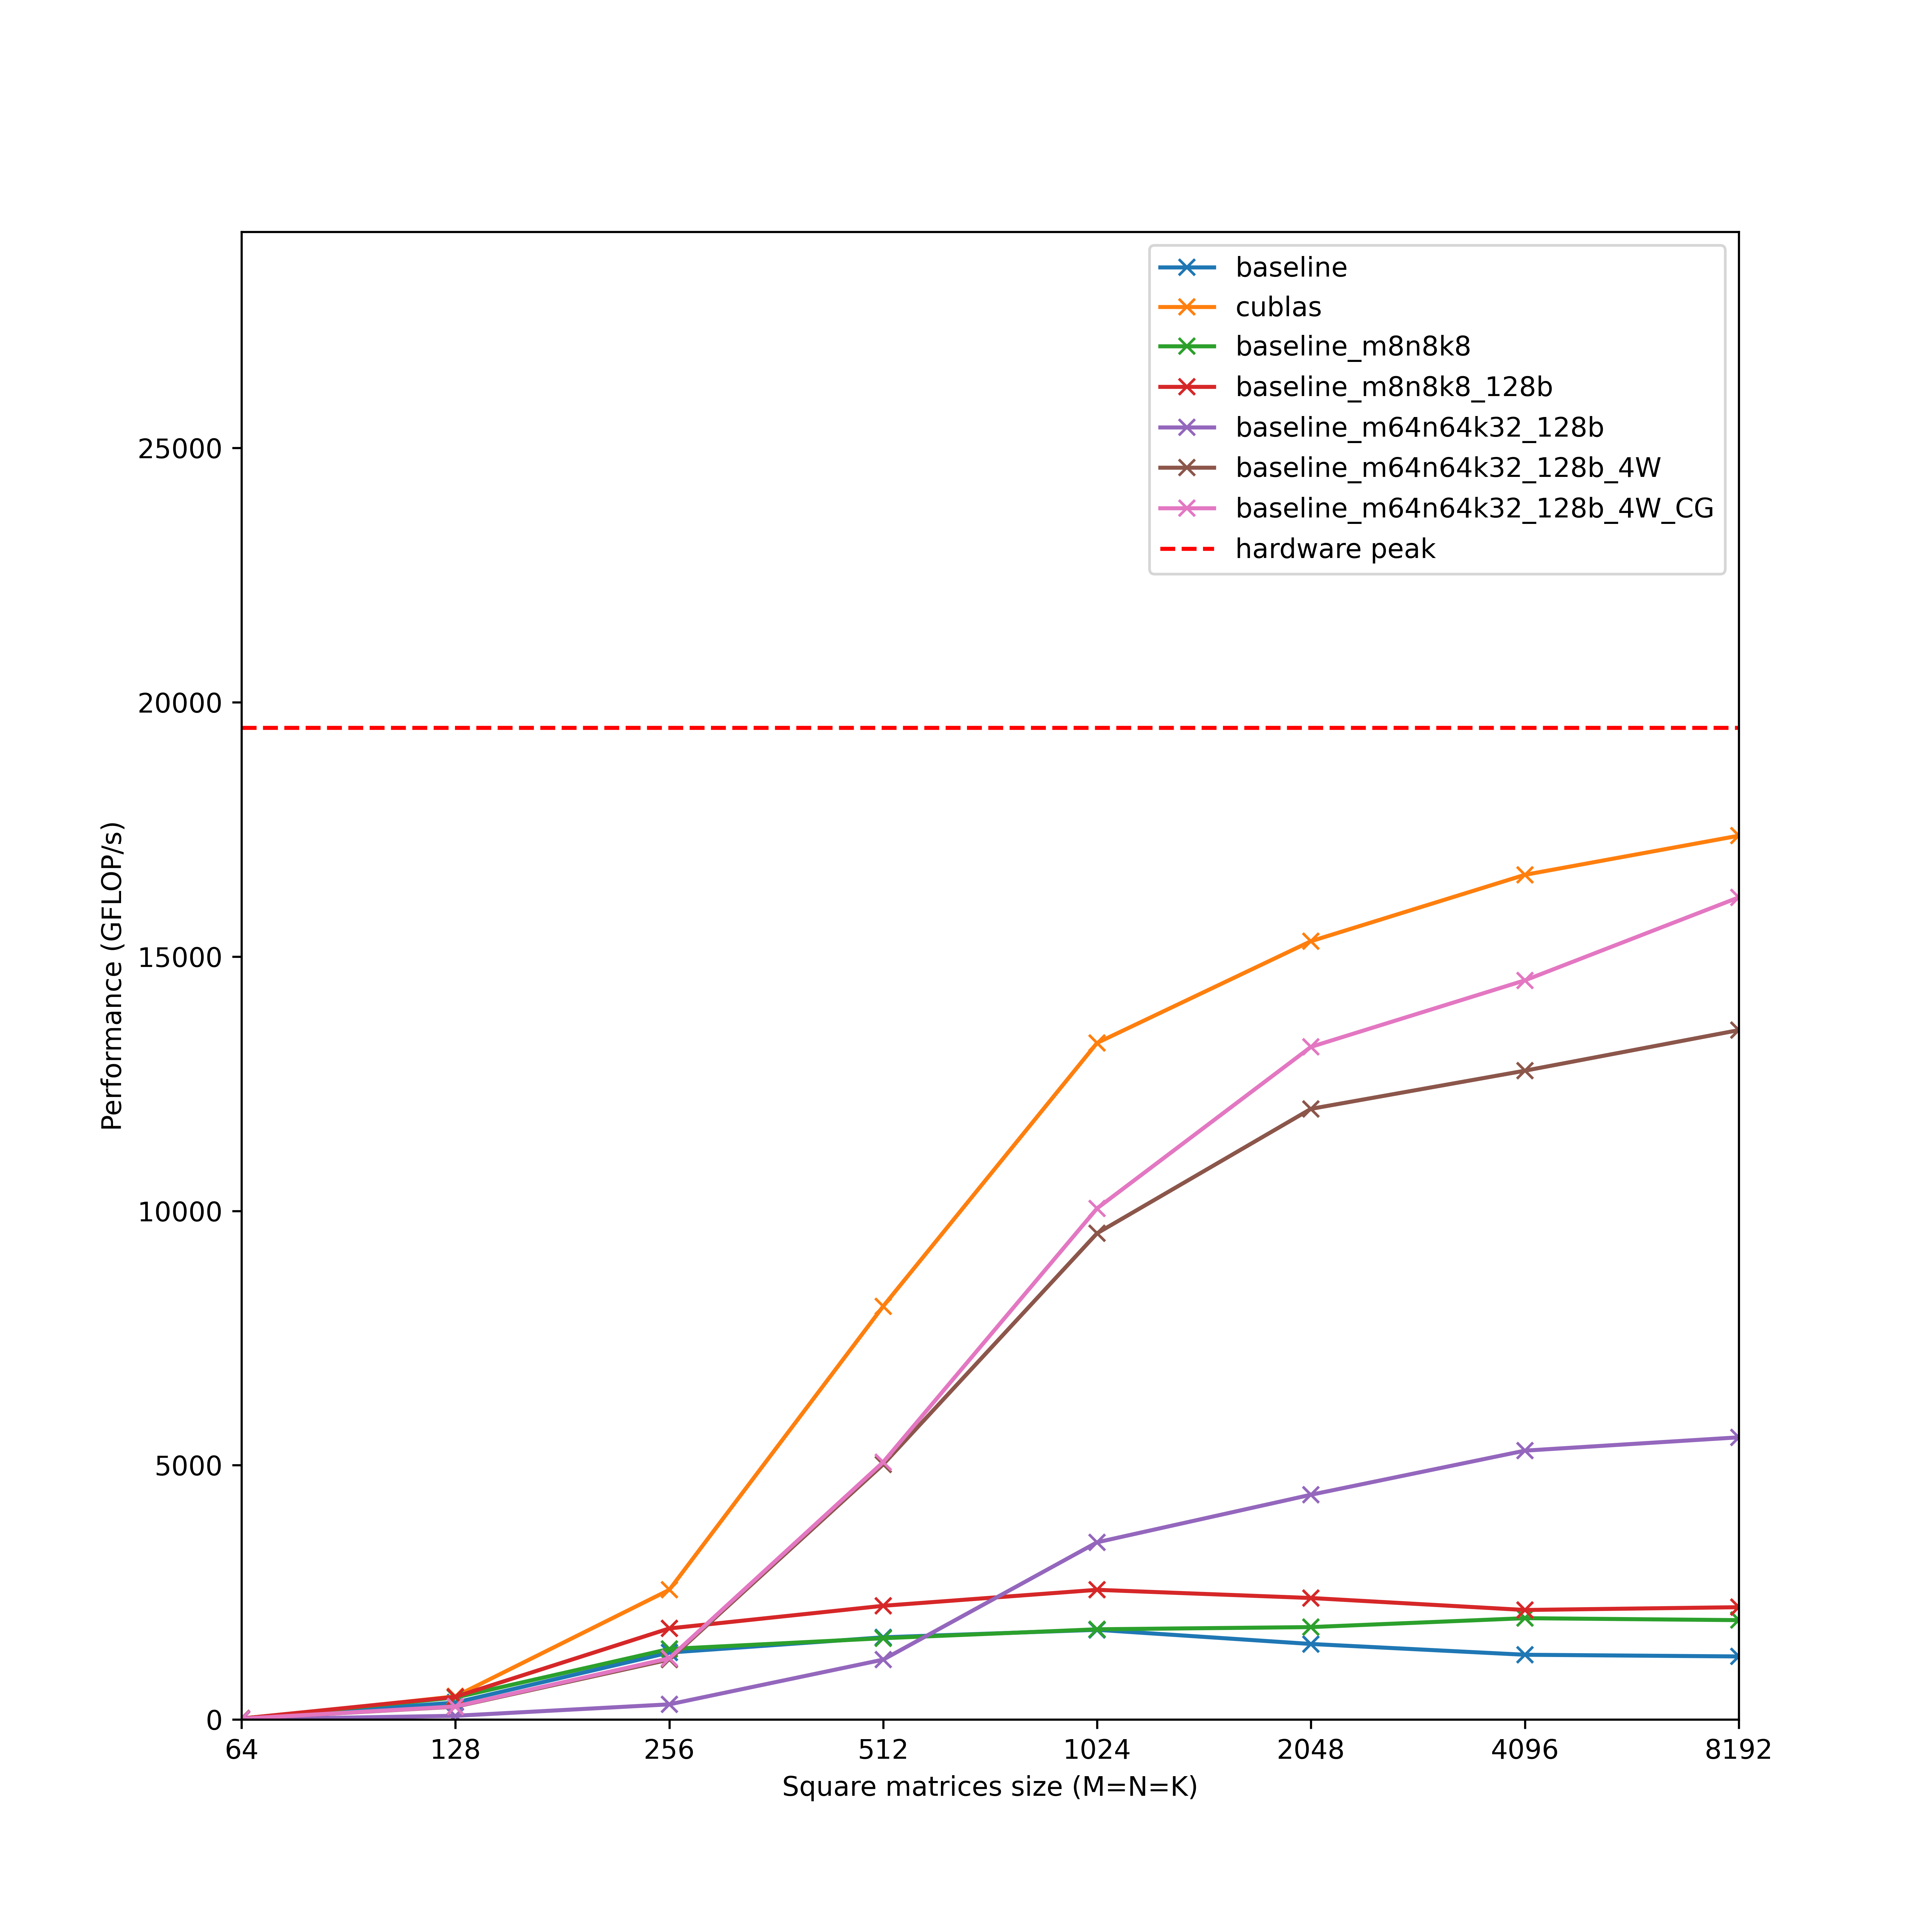
\includegraphics[width=0.5\textwidth]{assets/dgemm_cuda/cuda_baseline_m64n64k32_128b_4W_CG.png}
    \caption{Résultats de l'optimisation 5 (baseline\_m8n8k8\_128b\_4W\_CG) contre CuBLAS et la performance maximum théorique sur A100 SXM4.}
    \label{fig:baseline_m64n64k32_128b_4W_CG}
\end{figure}

Avec cette optimisation finale on arrive à 93\% (voir Figure \ref{fig:baseline_m64n64k32_128b_4W_CG}) de CuBLAS (16,2 sur 17,3 TFlops).


\subsection{Optimisations futures}

Avec les optimisations appliquées jusqu'à présent, on arrive à atteindre une performance respectable.
Cependant, les derniers pourcents sont les plus difficiles à avoir quand il s'agit de rattraper CuBLAS.

Avec plus de temps (ou de compétences en CuTe), nous aurions très certainement pu battre CuBLAS sur le DGEMM sur A100.
Le problème majeur de notre implémentation actuelle étant les copies de SMEM vers RMEM non vectorisées.
Nous n'avons pas réussi à forcer CuTe à permuter correctement les répétitions du microkernel pour avoir les 2 valeurs des paires de valeurs chargés par chaque thread contigues en mémoire (voir annexe \ref{appendix:smem_vectorized}).

CuBLAS n'est non plus parfaitement optimisé. Nous ne faisons pas de pipelining des copies depuis la mémoire globale vers la mémoire partagée ce que CuBLAS ne fait également pas.
Les optimisations basées sur une découverte dynamique du L2 (fragmenté en 2 parties, voir annexe \ref{}) ne semblent pas non plus faites.

Une explication peut être que la carte A100 SXM4 ne peut tout simplement pas produire plus d'opérations flottantes en réalité à cause de sa limite de puissance électrique (400W maximum).
Ce ne serait alors pas utile de plus optimiser le kernel puisque CuBLAS n'est ni memory bound ni compute bound mais bien power bound.
